\documentclass{beamer}
\usepackage{Config/style/uniReg}
\usepackage{tikz}
\usepackage{latexsym,amsmath,xcolor,multicol,booktabs,calligra}
\usepackage{hyperref}
\usepackage{subcaption}
\graphicspath{{figures/}}
\usetikzlibrary{positioning, arrows.meta, fit, shapes.geometric, calc}

% Use the theme color best suited for your departement. 
% Available themes (case sensitive) : Red, Yellow, GreenBrown, DarkBlue, Black&White (default)
\themecolor{Red}

% Change visibility of the logo in the background. Value can be 0, 1 or 2
\visibilitySiegel{0}

% title and subtitle
\title{Operator learning \newline for multi-patch domains}
\subtitle{}

% For multiple authors/presenters :
%   1. Comment \singleAuthor and use \multAuthors as in example
%   2. a- For same faculty/institute, you can use \AuthorInstitute{...}
%         instead if of \inst{...}
%      b- For different institutes, comment the line \AuthorInstitute{...} and use
%         \inst{...} together with \institute{...}
\singleAuthor{Massimiliano Ghiotto}
\AuthorInstitute{PhD student at University of Pavia}
%\multAuthors{Antoine Gansel\inst{1} \and Jullie Cailler\inst{2}}

%% collaborators with institute
% \Collaborators{{Julie Cailler\inst{2}}} 
% \Supervisors{Carlo Marcati\inst{1} \and {Giancarlo Sangalli\inst{1}}}
% \institute{{\inst{1}University of Pavia}}
%% collaborators without institute
\Supervisors{Carlo Marcati, \and Giancarlo Sangalli} % \institute{{\inst{1}University of Pavia}}

\newcommand{\numberset}{\mathbb}
\newcommand{\N}{\numberset{N}}
\newcommand{\Z}{\numberset{Z}}
\newcommand{\Q}{\numberset{Q}}
\newcommand{\R}{\numberset{R}}
\newcommand{\C}{\numberset{C}}

\begin{document}

\frame{\titlepage}

\addtocounter{framenumber}{-1}
\setbeamertemplate{footline}[footline-body]
\setbeamertemplate{background}[background-body]

%% ======================================

\section{Operator Learning}

%% ======================================

% \cite{kovachki2021neural}\blfootnote{\cite{kovachki2021neural}, Kovachki et al., "Neural operator: Learning maps between function spaces".}
\begin{frame}[t]{Definition of Neural Operator}
	\vspace{-0.5cm}
	\[ \mathcal{N}_{\theta} :\mathcal{A}(D, \R^{d_a}) \to \mathcal{U}(D, \R^{d_{u}}), \quad	\mathcal{N}_{\theta} := \mathcal{Q} \circ \mathcal{L}_L \circ \cdots \circ \mathcal{L}_1 \circ \mathcal{R} . \]
	\vspace{-0.2cm}
	\begin{enumerate}
		\item \textbf{Lifting:} linear and local operator 
			\[\mathcal{R}:\, \mathcal{A}(D, \R^{d_a}) \to \mathcal{U}(D, \R^{d_{v_1}}), \quad  \mathcal{R}(a)(x) = R\cdot a(x), \ R \in \R^{d_{v_1} \times d_a} \]
	\vspace{-0.2cm}
		\pause
		\item \textbf{Integral operator:} for $ t = 1, \dots, L $
		\[ \mathcal{L}_t : \, \mathcal{U}(D, \R^{d_{v_t}}) \to  \mathcal{U}(D, \R^{d_{v_{t}}}) \]
		\[  \mathcal{L}_t(v)(x) := \sigma\Big( W_t v(x)+ b_t(x) + (\mathcal{K}_t(a, \theta) v)(x) \Big) \]
		with $ \mathcal{K}_t(a, \theta) $ linear and non-local operator.  
		\pause
		\item \textbf{Projection:} linear and local operator 
		\[\mathcal{Q}:\, \mathcal{U}(D_{L}, \R^{d_{v_L}}) \to  \mathcal{U}(D, \R^{d_{u}}), \quad  \mathcal{Q}(v_L)(x) = Q\cdot v_L(x), \ Q \in \R^{d_{v_u} \times d_{v_L}}. \]		
	\end{enumerate}
\end{frame}

%% ======================================

\begin{frame}{Integral operator}
	There are different ways to define the integral operator $ \mathcal{K}_t $:
	\begin{itemize}
		\item defining $ \kappa_{t,\theta} \in C(D\times D,\, \R^{d_{v_{t}}\times d_{v_t}}) $
		\[ (\mathcal{K}_t(a, \theta)v_t)(x) = (\mathcal{K}_t(\theta)v_t)(x) = \int_{D} \kappa_{t,\theta}(x, y) v_{t}(y) \ d\mu_t(y).\]
		\pause
		\item defining $ \kappa_{t,\theta} \in C(D\times D\times \R^{d_a} \times \R^{d_a},\, \R^{d_{v_{t}}\times d_{v_t}}) $
		\[	(\mathcal{K}_t(a, \theta)v_t)(x) = \int_{D} \kappa_{t, \theta}\left( x, y, a\left(x\right), a\left(y\right) \right)v_t(y)  \ d\mu_t(y).\]
		\pause
		\item defining $ \kappa_{t,\theta} \in C(D\times D\times \R^{d_{v_t}} \times \R^{d_{v_t}},\, \R^{d_{v_{t}}\times d_{v_t}}) $
		\[ (\mathcal{K}_t(a, \theta)v_t)(x) = \int_{D} \kappa_{t,\theta}\left( x, y, v_{t}\left(x\right), v_t(y) \right) v_t(y)  \ d\mu_t(y). \]
	\end{itemize}
\end{frame}

%% ======================================

% \begin{frame}
% 	% \blfootnote{\cite{kovachki2021neural}, Kovachki et al., "Neural operator: Learning maps between function spaces".}
% 	\begin{themedTitleBlock}{Teorema}%\cite{kovachki2021neural}
% 		Sono casi particolari di operatori neurali:
% 		\begin{itemize}
% 			\item le reti neurali classiche;
% 			\item le reti neurali convoluzionali;
% 			\item i transformers;
% 			\item le DeepONets;
% 		\end{itemize}
% 	\end{themedTitleBlock}
% \end{frame}

%% ======================================
\section{Fourier Neural Operator}
%% ======================================

\begin{frame}{Definition of Fourier Neural Operator (FNO)}
	For defining the Fourier Neural Operator we make the first assumption and the further assumption that $\kappa_{t,\theta}(x, y) = \kappa_{t,\theta}(x -y)$,
	\[ (\mathcal{K}_t(a, \theta)v)(x) = \int_{\mathbb{T}^d} \kappa_{t,\theta}(x-y) v(y) \ dy = (\kappa_{t, \theta} * v)(x)  .\]
	Using the convolution theorem we have
	\[ (\kappa_{t, \theta} * v)(x) =  \mathcal{F}^{-1}\left( \mathcal{F}( \kappa_{t,\theta}) (k) \cdot \mathcal{F}(v)(k) \right)(x), \]
	and parameterizing $\mathcal{F}( \kappa_{t, \theta} )$ with the parameters $P_{\theta}(k) \in \C^{d_v \times d_v} \ \forall k $ we have  
	\[  (\mathcal{K}_t(a, \theta)v)(x)= \mathcal{F}^{-1}\left( P_{\theta}(k) \cdot \mathcal{F}(v)(k) \right)(x) \]
\end{frame}

%% ======================================

\begin{frame}{Fourier Neural Operator}
    \begin{center}
    \begin{tikzpicture}
        \tikzset{
            box/.style={draw, rounded corners, align=center, minimum height=0.8cm, minimum width=1cm, fill=orange!30},
            bigbox/.style={draw, rounded corners, align=center, minimum height=2cm, minimum width=1cm, fill=yellow!30},
            node_sum/.style={draw, circle, fill=white, inner sep=0pt, minimum size=4mm},
            every node/.style={font=\small}
        }
        % Nodes for the main structure
        \node[box, label=above:{\textit{Input}}] (input) {$f(x)$};
        \node[box, right=0.5cm of input, label=above:{\textit{Lifting}}] (lifting) { $\mathcal{P}$ };
        \node[bigbox, right=0.5cm of lifting] (fourier1) {$\mathcal{L}_{1}$};
        \node[bigbox, right=0.55cm of fourier1] (fourier2) {$\mathcal{L}_{t}$};
        \node[bigbox, right=0.55cm of fourier2] (fourier3) {$\mathcal{L}_{L}$};
        \node[box, right=0.5cm of fourier3, label=above:{\textit{Projection}}] (projection) {$\mathcal{Q}$};
        \node[box, right=0.5cm of projection, label=above:{\textit{Output}}] (output) {$u(x)$};
        
        % Draw arrows between nodes
        \draw[->, line width = .7pt] ($(input.east)+(0.05, 0)$) -- ($(lifting.west)-(0.05,0)$);
        \draw[->, line width = .7pt] ($(lifting.east)+(0.05, 0)$) -- ($(fourier1.west)-(0.03,0)$);
        \draw[dotted, line width = 2pt] ($(fourier1.east)+(0.1, 0)$) -- ($(fourier2.west)-(0.1,0)$);
        \draw[dotted, line width = 2pt] ($(fourier2.east)+(0.1, 0)$) -- ($(fourier3.west)-(0.1,0)$);
        \draw[->, line width = .7pt] ($(fourier3.east)+(0.05, 0)$) -- ($(projection.west)-(0.05,0)$);
        \draw[->, line width = .7pt] ($(projection.east)+(0.05, 0)$) -- ($(output.west)-(0.05,0)$);
        
        % Annotations for the Fourier Layers
        \node[align=center, above=0.2cm of fourier2, font=\footnotesize] { \textit{Fourier Layers} };
        
        % Internal structure bounding box
        \node[draw, line width = .7pt, rounded corners, inner sep=0.2cm, fit= (fourier1) (fourier2) (fourier3)] (internal) {};

        %%% Second part of the plot
        % Internal structure bounding box
		\node[draw, below=0.2cm of internal, rounded corners, inner sep=0.2cm, fill=yellow!30] (internal) {
			\begin{tikzpicture}[every node/.style={font=\small}]
				% Nodes for the internal structure
				\node[box] (vt) {$v_{t}(x)$};
				\node[box, right=1cm of vt] (transform) {$\mathcal{F}$};
				\node[box, right=0.5cm of transform, fill=green!25] (nonlinear) { $ R_{\theta_t} $ };
				\node[box, right=0.5cm of nonlinear] (invtransform) { $ \mathcal{F}^{-1} $ };
				\node[box, below=0.8cm of nonlinear, fill=green!25] (linear) { $ W_t, b_t $ };

                % Internal structure bounding box
                \node[draw, line width = .7pt, rounded corners, inner sep=0.15cm, fit= (transform) (nonlinear) (invtransform) ] (diagonalscaling) {};

				\node[node_sum, right=0.5cm of invtransform] (node_sum) {$\mathbf{+}$};
				\node[box, right=0.5cm of node_sum] (activation) {$\sigma$};
				\node[box, right=0.5cm of activation] (vtplusone) {$v_{t+1}(x)$};
				
				% Draw arrows between nodes
				\draw[line width = .7pt] ($(vt.east)+(0.05, 0)$) -- (diagonalscaling);
				\draw[->, line width = .7pt] ($(transform.east)+(0.05, 0)$) -- ($(nonlinear.west)-(0.05, 0)$);
				\draw[->, line width = .7pt] ($(nonlinear.east)+(0.05, 0)$) -- ($(invtransform.west)-(0.05, 0)$);
				\draw[->, line width = .7pt] ($(vt.south)-(0, 0.05)$) |- ($(linear.west)-(0.05, 0)$);
				\draw[->, line width = .7pt] (diagonalscaling) -- ($(node_sum.west)-(0.05, 0)$);
				\draw[->, line width = .7pt] ($(linear.east)+(0.05, 0)$) -| ($(node_sum.south)-(0, 0.05)$);
				\draw[->, line width = .7pt] ($(node_sum.east)+(0.05, 0)$) -- ($(activation.west)-(0.05, 0)$);
				\draw[->, line width = .7pt] ($(activation.east)+(0.05, 0)$) -- ($(vtplusone.west)-(0.05, 0)$);

			\end{tikzpicture}
		};
        % Connection between the two parts
        \draw[] ($(internal.north west)+(0.1, 0.05)$) -- (fourier2.south west);
        \draw[] ($(internal.north east)+(-0.1, 0.05)$) -- (fourier2.south east);
    \end{tikzpicture}
    \end{center}
\end{frame}

%% ======================================

\begin{frame}{}% \blfootnote{\cite{kovachki2021universal}, Kovachki et al., "On universal approximation and error bounds for fourier neural operators".}
\begin{themedTitleBlock}{Teorema di approssimazione universale per le FNO} % \cite{kovachki2021universal}
	Siano $ s, s' \ge 0 $ e 
	\[ \mathcal{G}: H^s(\mathbb{T}^d, \R^{d_a}) \to H^{s'}(\mathbb{T}^d, \R^{d_u}) \]
	un operatore continuo. Siano $ K \subset H^s(\mathbb{T}^d, \R^{d_a}) $ un insieme compatto e $ \sigma \in \C^{\infty}(\R) $ funzione di attivazione  non polinomiale e globalmente Lipschitz. Allora, per ogni $ \varepsilon > 0 $, esiste un operatore continuo con struttura data da una FNO 
	\[ \mathcal{N}: H^s(\mathbb{T}^d, \R^{d_a}) \to H^{s'}(\mathbb{T}^d, \R^{d_u}) \]
	tale che:
	\[ \underset{a \in K}{sup}\, \left\| \mathcal{G}(a) - \mathcal{N}(a) \right\|_{H^{s'}} \le \varepsilon.  \]
\end{themedTitleBlock}	
\end{frame}

%% ======================================

\begin{frame}{Pseudo Operatori Neurali di Fourier ($ \psi $-FNO)}
	Uno pseudo-operatore di Fourier è una mappa
	\[ \mathcal{N}^{*}: \mathcal{A}(\mathbb{T}^d, \R^{d_a}) \to \mathcal{U}(\mathbb{T}^d, \R^{d_u}), \qquad a \mapsto \mathcal{N}^{*}(a), \]
	della forma
	\[\mathcal{N}^{*}(a) = \mathcal{Q} \circ I_N \circ \mathcal{L}_L \circ I_N \circ \dots \circ \mathcal{L}_1 \circ I_N \circ \mathcal{R}(a),	\]
	dove $ I_N $ denota la proiezione pseudo-spettrale di Fourier di grado $ N $
	\[ I_N : C(\mathbb{T}^d) \to L^{2}_{N}(\mathbb{T}^{d}), \quad u \mapsto I_Nu. \]
	Uno $ \psi $-FNO si può identificare con una mappa finita dimensionale
	\[ \widetilde{\mathcal{N}}^{*}: \R^{d_a \times \mathcal{I}_N} \to \R^{d_a \times \mathcal{I}_N}, \quad \widetilde{\mathcal{N}}^{*}:a \mapsto \widetilde{\mathcal{N}}^{*}(a)  \]
	\[ \widetilde{\mathcal{N}}^{*}(a)_j = \mathcal{N}^{*}(a)(x_j) \]
\end{frame}
%% ======================================

\begin{frame}
	% \blfootnote{\cite{kovachki2021universal}, Kovachki et al., "On universal approximation and error bounds for fourier neural operators".}
	\vspace{-0.2cm}
	\begin{themedTitleBlock}{Teorema di approssimazione universale per le $ \psi $-FNO } %\cite{kovachki2021universal}
		Siano $ s > d/2$ , $ s' \ge 0 $ e 
		\[ \mathcal{G}: H^s(\mathbb{T}^d, \R^{d_a}) \to H^{s'}(\mathbb{T}^d, \R^{d_u}) \]
		un operatore continuo. Siano $ K \subset H^s(\mathbb{T}^d, \R^{d_a}) $ un insieme compatto e $ \sigma \in \C^{\infty}(\R) $ una funzione di attivazione non polinomiale e globalmente Lipschitz. Allora, per ogni $ \varepsilon > 0 $, esiste un $ N \in \N $ tale che la $ \psi $-FNO 
		\[ \mathcal{N}^{*}: L^2_N(\mathbb{T}^d, \R^{d_a}) \to L^2_N(\mathbb{T}^d, \R^{d_u}) \]
		soddisfa:
		\[ \underset{a \in K}{sup}\, \left\| \mathcal{G}(a) - \mathcal{N}^{*}(a) \right\|_{H^{s'}} \le \varepsilon.  \]
	\end{themedTitleBlock}	
\end{frame}
%% ======================================

\begin{frame}
	% \blfootnote{\cite{kovachki2021universal}, Kovachki et al., "On universal approximation and error bounds for fourier neural operators".}
	\vspace{-0.2cm}
	\begin{themedTitleBlock}{Teorema} % \cite{kovachki2021universal}
		Sia $ s > d/2 $, $ \lambda \in (0,1) $ e consideriamo l'operatore soluzione del problema di Darcy
		\[ \mathcal{G}: \mathcal{A}_{\lambda}^{s}(\mathbb{T}^d) \to H^1(\mathbb{T}^d). \]
		Fissata $ \sigma \in C^3(\R) $ non polinomiale per ogni $ N \in \N $ esiste $ C > 0 $ e una $ \psi $-FNO
		\[ \mathcal{N}^{*}: \mathcal{A}_{\lambda}^{s}(\mathbb{T}^d) \to H^1(\mathbb{T}^d)  \]
		tale che
		\[ \underset{a \in \mathcal{A}_{\lambda}^{s}}{sup} \left\| \mathcal{G}(a) - \mathcal{N}^{*}(a) \right\|_{H^1(\mathbb{T}^d)} \le CN^{-k} \]
		e $\ \mathrm{depth}(\mathcal{N}^{*}) \le C \log(N) $, $\  \mathrm{lift}(\mathcal{N}^{*}) \le C $, $\ \mathrm{size}(\mathcal{N}^{*}) \lesssim N^d\log(N). $
	\end{themedTitleBlock}
\end{frame}
%% ======================================

\section{Problema di Darcy}
%% ======================================

\begin{frame}{Problema di Darcy}
	\[ 	\begin{cases}
		- \nabla(a \cdot \nabla u) = f,\quad &  \mathrm{in}\ D\\
		u = 0, & \mathrm{on} \ \partial D
	\end{cases} \]
	con $ D = [0, 1]^2 $, $\ \mathcal{A} = L^{\infty}(D, \R^+) $, $\ \mathcal{U} = H^1_0(D, \R) $ e $\ f \equiv 1 $.
	\[  \mathcal{G}: L^{\infty}(D, \R^+) \to H^1_0(D, \R), \qquad \mathcal{G}:a \mapsto u. \]
	\begin{figure}
		\centering
		\begin{subfigure}{0.4\textwidth}
			\centering
			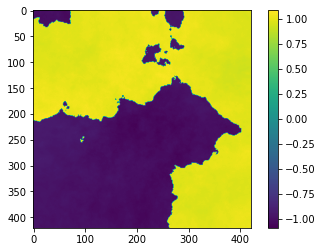
\includegraphics[width=\textwidth]{zero-shot-coeff.png}
			\caption{Coefficiente}
		\end{subfigure}
		\hfill
		\begin{subfigure}{0.4\textwidth}
			\centering
			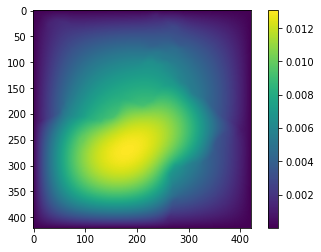
\includegraphics[width=\textwidth]{zero-shot-sol.png}
			\caption{Sol. esatta}
		\end{subfigure}
	\end{figure}
\end{frame}
%% ======================================

\begin{frame}{Norma relativa $ L^2 $}
	\[ \left\| \frac{\mathcal{G} - \mathcal{N}^{*}_{\theta}}{\mathcal{G}}\right\|_{L_{\mu}^2(L^{\infty}, L^{2})} = 	\mathbb{E}_{a \sim \mu} \frac{\left\| \mathcal{G}(a) - \mathcal{N}^{*}_{\theta}(a) \right\|^{2}_{L^2(D)}}{\left\| \mathcal{G}(a)\right\|^{2}_{L^2(D)}} \approx \]
	\[\approx \frac1N \sum_{i=1}^{N}\left(  \frac{\sum_{k=1}^{M} \left| u^{(i)}\left( x_k\right)  - \widetilde{\mathcal{N}}^{*}_{\theta}\left(a^{(i)}\right)\left( x_k\right)  \right|^{2}}{\sum_{k=1}^{M}\left| u^{(i)}\left( x_k\right)  \right|^{2}}\right)	\]
	con $ D_k = \left\lbrace x_{k} \right\rbrace_{k = 1}^{M} \subset D = [0, 1]$ e $ M = 85^2 $. Dataset $ \left\lbrace a^{(i)}, u^{(i)} \right \rbrace_{i=1}^{N} $ con $ a^{(i)} \sim\mu = T_{\#}N(0, C) $ i.i.d. e $ u^{(i)} = \mathcal{G}(a^{(i)}) $ soluzione approssimata e con valutazioni puntuali $ \left\lbrace a^{(i)}_{|D_k}, u^{(i)}_{|D_k} \right \rbrace_{i=1}^{N} $.
\end{frame}
%% ======================================

\begin{frame}
	\begin{figure}[h!!]
		\centering
		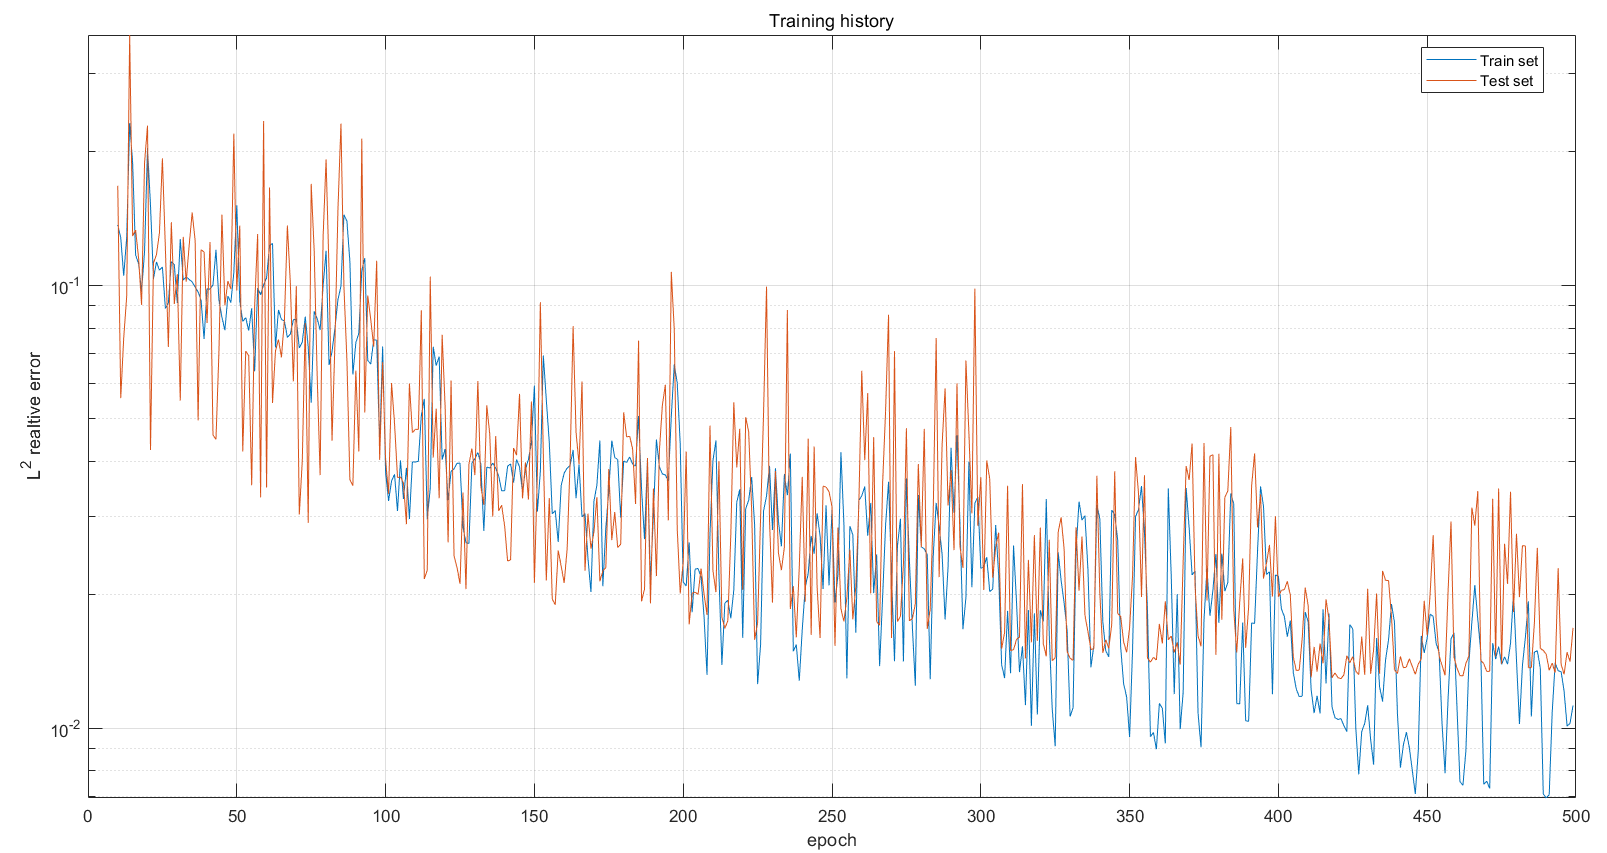
\includegraphics[width=0.65\textwidth]{DarcyFNO_L4_train.png}
	\end{figure}
	Griglia $ 85 \times 85 $ con $ L=4 $, $ d_v = 32 $, $ k_{max} = 12 $, $ \sigma = ReLU $, $ 1000 $ funzioni per l'allenamento e $ 200 $ per il test, $ 500 $ epoche e learning rate inizializzato a $ 0,001 $ e dimezzato ogni $ 100 $ epoche.
	\begin{table}[h!] %booktabs
		\centering
		\begin{tabular}{cccc}\toprule
			train error & rel. error $ L^2 $ & parameters & training time \\
			\cmidrule{1-4}
			$ 0.01305 $ & $ 0.01804 $ & $ 2 \, 363 \, 681  $ & $ 6 $ hours\\
			\bottomrule
		\end{tabular}
	\end{table}
\end{frame}
%% ======================================

\begin{frame}{Norma relativa $ H^1 $}
	\[ \left\| \frac{\mathcal{G} - \mathcal{N}^{*}_{\theta}}{\mathcal{G}}\right\|_{L_{\mu}^2(L^{\infty}, H^{1}_0)} = \mathbb{E}_{a \sim \mu} \frac{\left\| \mathcal{G}(a) - \mathcal{N}^{*}_{\theta}(a) \right\|^{2}_{H^1(D)}}{\left\| \mathcal{G}(a)\right\|^{2}_{H^1(D)}},  \]
	dove \[ \left\| f \right\|_{H^1(\mathbb{T}^d)}^2 = \sum_{k \in \Z^d}	\left(1+|k|^2	\right)^s \left| \widehat{f}(k) \right|^2 \]
	da cui
	\[\left\| \frac{\mathcal{G} - \mathcal{N}^{*}_{\theta}}{\mathcal{G}}\right\|_{L^2_{\mu}(L^{\infty}, H^{1}_0)} \approx\]\[ \approx \frac1N \sum_{i=1}^{N} \frac{\sum_{k \in \Z_{N}}	\left(1+|k|^2 \right)^s \left| \widehat{u^{(i)}}(k) - \widehat{\mathcal{N}_{\theta}^{*}\left(a^{(i)}\right)}(k)\right|^2} {\sum_{k \in \Z_{N}}\left(1+|k|^2	\right)^s \left| \widehat{u^{(i)}}(k) \right|^2}	 \]
\end{frame}
%% ======================================

\begin{frame}{}
	\small La norma relativa $ H^1 $ come funziona di perdita aiuta l'allenamento dell'operatore neurale.
	\begin{table}[h!] %booktabs
		\centering
		\begin{tabular}{ccc}\toprule
			funzione di perdita & errore rel. $ L^2 $ & errore rel.  $ H^1 $ \\
			\cmidrule{1-3}
			rel. $ L^2 $ & $ 0.01804 $ & $ 0.06944 $\\
			rel. $ H^1 $ & $ 0.01203 $& $ 0.04793 $  \\
			\bottomrule
		\end{tabular}
	\end{table}
	{\small Nuove prestazioni con la norma relativa $ H^1 $ come funzione di perdita.}
	\begin{table}[h!] %booktabs
		\centering
		\begin{tabular}{ccc}\toprule
			funzione di perdita &  errore rel. $ L^2 $ & errore rel.  $ H^1 $ \\
			\cmidrule{1-3}
			rel. $ L^2 $ & $ 0.01038 $ & $ 0.05979  $ \\
			rel. $ H^1 $ & $ \mathbf{0.007220} $ & $ \mathbf{0.03803}  $ \\
			\bottomrule
		\end{tabular}
	\end{table}
	{\small Entrambe le architetture hanno $ 2\, 376\, 449 $ parametri ed impiegano $ 7 $ ore per l'allenamento.}
	% \cite{li2020fourier} \blfootnote{\cite{li2020fourier}, Li et al., "Fourier neural operator for parametric partial differential equations".}
\end{frame}
%% ======================================

\section{Multi-patch domains}
%% ======================================

\begin{frame}{Problema di Darcy su un dominio ad L}
	\[ 	\begin{cases}
		- \nabla(a \cdot \nabla u) = f,\quad &  \mathrm{in}\ \Omega\\
		u = 0, & \mathrm{in} \ \partial\Omega
	\end{cases} \]
	problema di Darcy su $ \Omega = [-1,1]^2\setminus(0,1)\times (-1,0) $, $ f \equiv 1 $.
	\begin{figure}
		\centering
		\begin{subfigure}{0.36\textwidth}
			\centering
			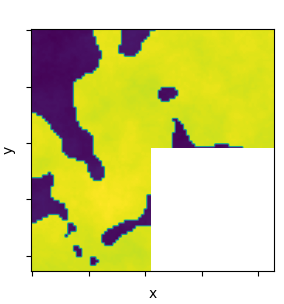
\includegraphics[width=\textwidth]{CoefficientiL.png}
			\caption{Coefficiente}
		\end{subfigure}
		\hfill
		\begin{subfigure}{0.45\textwidth}
			\centering
			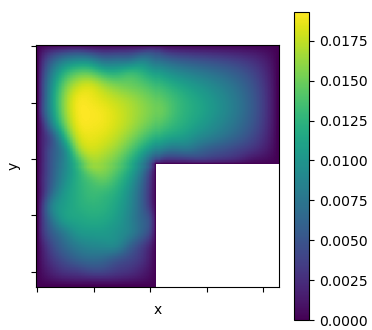
\includegraphics[width=\textwidth]{SoluzioneL.png}
			\caption{Sol. esatta}
		\end{subfigure}
	\end{figure}
\end{frame}
%% ======================================

\begin{frame}{Fourier continuation}
	Gli operatori neurali di Fourier hanno la limitazione che sono ristretti a domini rettangolari. Quando ho un dominio irregolare posso estenderlo a un dominio rettangolare più grande, la funzione di perdita calcolata solo sul dominio originale.
	\begin{table}[h!] %booktabs
		\centering
		\begin{tabular}{ccc}\toprule
		errore rel. $ L^2 $ & parametri & tempo allenamento \\
			\cmidrule{1-3}
			$ 0.02450 $ & $ 2\, 363\, 681 $ & $ 7 $ hours\\
			\bottomrule
		\end{tabular}
	\end{table}
	\begin{figure}
		\centering
		\begin{subfigure}{0.45\textwidth}
			\centering
			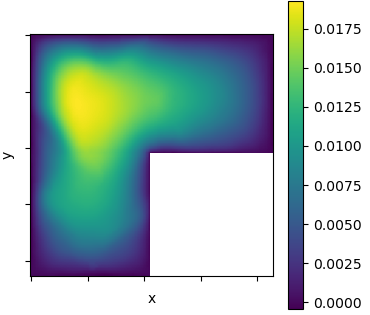
\includegraphics[width=0.8\textwidth]{SoluzioneContinuationL.png}
		\end{subfigure}
		\hfill
		\begin{subfigure}{0.45\textwidth}
			\centering
			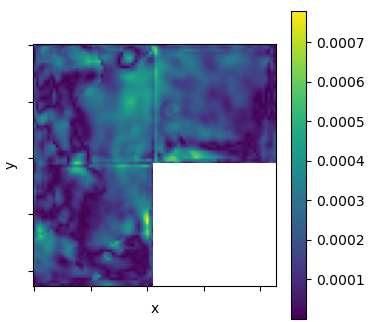
\includegraphics[width=0.8\textwidth]{DifferenzaContinuationL.png}
		\end{subfigure}
	\end{figure}
\end{frame}
%% ======================================

% \begin{frame}[noframenumbering]{Bibliografia}
% 	\nocite{*}
% 	\printbibliography
% \end{frame}

%% ======================================
\backmatter % last slide

\appendix
\begin{frame}[noframenumbering]{Trasformata di Fourier}
	\centering
	\begin{itemize}
		\item  Sia $ v \in  L^2(\mathbb{T}^d) $, la trasformata di Fourier è
		\[ \begin{split}
			\mathcal{F} : \ & L^{2}(\mathbb{T}^d, \C^{n})\to \ell^{2}(\Z^d, \C^{n})\\
			& v \mapsto \mathcal{F}(v)
		\end{split} \]
		\[ \mathcal{F}(v)(k) := \frac{1}{(2 \pi)^{d}} \int_{\mathbb{T}^{d}}v(x) e^{-i \left\langle k , x \right\rangle} \ dx,  \quad \forall k \in \Z^d. \]
		\item Data $ \widehat{v} = \left\lbrace \widehat{v}_k\right\rbrace_{k \in \Z^d} \in \ell^{2}(\Z^d, \C^{n}) $, la trasformata inversa di Fourier è
		\[ \begin{split}
			\mathcal{F}^{-1} : \ & \ell^{2}(\Z^d, \C^{n}) \to L^{2}(D, \C^{n})\\
			& \widehat{v} \mapsto \mathcal{F}^{-1}(\widehat{v})
		\end{split} \]
		\[ (\mathcal{F}^{-1}\widehat{v})(x) = \sum_{k \in \Z^d} \widehat{v}_k e^{i \left\langle k , x \right\rangle } \qquad \forall x \in D. \]
	\end{itemize}
\end{frame}

\begin{frame}[noframenumbering]{Trasformata discreta di Fourier}
	Sia $ N \in \N $ e fissata una griglia regolare $ \{x_j\}_{j \in \mathcal{I}_N} $ con $ x_j = (2\pi j)/(2N+1) \in \mathbb{T}^d $, $ j \in \mathcal{I}_N = \{0, \dots, 2N\}^{d} $ e scelto un insieme per i modi di Fourier $\mathcal{K}_N := \{k \in \Z^d : |k|_{\infty} \le N\}$.
	Definiamo la trasformata discreta di Fourier come
	\[ \mathcal{F}_{N}: \R^{\mathcal{I}_N} \to \C^{\mathcal{K}_N}\]\[ \mathcal{F}_{N}(v)(k) := \frac{1}{(2N+1)^{d}} \sum_{j \in \mathcal{I}_N}v(x_j) e^{-2\pi i \left\langle j, k \right\rangle/N }, \quad \forall k \in \mathcal{K}_N, \]
	e la trasformata inversa discreta di Fourier come
	\[ \mathcal{F}_{N}^{-1}: \C^{\mathcal{K}_N} \to \R^{\mathcal{I}_N}\]\[ \mathcal{F}_{N}^{-1}(\widehat{v})(j) := \sum_{k \in \mathcal{K}_N} \widehat{v}_k e^{2\pi i \left\langle j, k \right\rangle/N }, \qquad \forall j \in \mathcal{J}_N. \]
\end{frame}

\begin{frame}[noframenumbering]{Schema dimostrazione teo. universale FNO}
	\centering
	\begin{itemize}
		\item Proiezione sullo spazio dei polinomi trigonometrici
		\[ P_N: L^{2}(\mathbb{T}^d) \to L^{2}_N(\mathbb{T}^d),  \]
		\[ P_N\left(\sum_{k \in \Z^d} c_k e^{i \left\langle x, k \right\rangle } \right) = \sum_{|k|_{\infty}\le N} c_k e^{i \left\langle x, k \right\rangle }, \qquad \forall (c_k)_{k \in \Z^d} \in \ell^2(\Z^d). \]
		\item Se il teorema universale vale per $ s'=0 $ allora vale per per qualsiasi valore di $ s' \ge 0 $.
		\item Fissiamo $ s' = 0 $  \[ \mathcal{G}_{N}: H^{s}(\mathbb{T}^d, \R^{d_a}) \to L^2(\mathbb{T}^d, \R^{d_u}), \qquad \mathcal{G}_{N}(a):= P_N  \mathcal{G} (P_Na), \]
		vale che $ \forall \varepsilon > 0 $, $ \exists N \in \N $ si ha
		\[ \left\|\mathcal{G}(a) - \mathcal{G}_N(a) \right\|_{L^2} \le \varepsilon, \qquad \forall a \in K. \]
	\end{itemize}
\end{frame}

\begin{frame}[noframenumbering]{Schema dimostrazione teo. universale FNO}
	Definiamo l'operatore
	\[ \widehat{\mathcal{G}}_N: \C^{\mathcal{K}_N} \to\C^{\mathcal{K}_N}, \qquad \widehat{\mathcal{G}}_N(\widehat{a}_k) := \mathcal{F}_N (\mathcal{G}_N ( Re (\mathcal{F}_N^{-1}(\widehat{a}_k)))), \]
	per il quale vale l'identità
	\[ \mathcal{G}_N (a) = \mathcal{F}_N^{-1} \circ \widehat{\mathcal{G}}_N \circ \mathcal{F}_N (P_Na), \]
	per le funzioni $  a \in L^2(\mathbb{T}^d, \R^{d_a}) $. Ci si riconduce a dimostrare che gli operatori neurali di Fourier possono approssimare
	\[ \mathcal{F}_N^{-1}, \ \widehat{\mathcal{G}}_N , \ \mathcal{F}_N (P_Na). \]
\end{frame}

\begin{frame}[noframenumbering]{Definizione MLP}
	Let $ d \in \N $ and $ L\in \N $ with $ L \ge 2 $ and $ \sigma : \R \to \R  $ an activation function. Let $ A_{\ell} \in \R^{n_{\ell}\times n_{\ell-1}} $, $ b_{\ell} \ in \R^{\ell} $ with $ n_{\ell}\in \N $ for $ \ell = 1, \dots, L $	and $ n_{0} = d $. We call multilayer perceptron (MLP) the function defined as
	\[ \begin{cases}
		x_{L} = A_{L}x_{L-1} + b_{L} \qquad & \\
		x_{\ell} = \sigma\left( A_{\ell}x_{\ell-1} + b_{\ell} \right) 
	\end{cases}, \]
	where $ x_0 $ is the input and $ x_{L} $ is the output of the function.
\end{frame}

\begin{frame}[noframenumbering]{Universal approximation theorem for operator}
	Suppose that $ \sigma \in TW $, $ X $ is a Banach space, $ K_1 \subset X $, $ K_2 \subset \R^d $ are two compact sets in $ X $ and $ \R^{d} $ respectively, and $ V $ is a compact set in $ C(K_1) $. Let $ G $ a nonlinear continuous operator which maps $ V $ into $ C(K_2) $, then for any $ \varepsilon > 0 $, there are a positive integers $ n $, $ p $, $ m $; real constants $ c_i^{k}$, $ \theta_i^{k}$, $ \xi_{ij}^{k} $, $ \zeta^k \in \R $, points $ w^{k} \in \R^d $ and $ x_j \in K_1 $, with $ i = 1, \dots, n$, $ j = 1, \dots, m $ and $ k = 1, \dots, p $, such that
	\[ \left| G(u)(y) - \sum_{k=1}^{p}\sum_{i=1}^{n}c_i^k \sigma \left( \sum_{j=1}^{m} \xi_{ij}^k u(x_j) + \theta_i^k \right) \sigma(w^k \cdot y + \zeta^k) \right| < \varepsilon  \]
	holds for all $ u \in V $ and $ y \in K_2 $.
\end{frame}

\end{document}


To begin a  new line with some fixed vertical space
\vspace{\baselineskip}

\begin{block}{title}
\end{block}


% \begin{verbatim}  This begins a verbatim environment where the text is displayed exactly as it is written. This is useful for showing code snippets


% \begin{itemize}[<+->]  This starts an itemized (bulleted) list. The [<+->] option specifies that each item in the list should be revealed one by one as the presentation progresses (incrementally).


% \begin{frame}[fragile]{Writing a Simple Slide}  This starts a new slide (frame) titled "Writing a Simple Slide". The fragile option is used because the frame will contain verbatim text, which needs special handling in Beamer.


\uncover<2->{ <content> }  this means that the `content` is veasible from the second transition of the slide
The \uncover command makes the text visible starting from the specified slide number.


\begin{columns} % adding [onlytextwidth] the left margins will be set correctly
    \begin{column}{0.50\textwidth}
        
    \end{column}%
    \begin{column}{0.50\textwidth}
        
    \end{column}
\end{columns}


\textcolor{<color name>}{text}, \emph{}, \alert{} --> commands to brings the attention somewhere


% for a single monocrome block
\begin{themedColorBlock}{ `title` }
    `content`
\end{themedColorBlock}


% for block with highlighted title
\begin{themedTitleBlock}{ `title` }
    `content`
\end{themedTitleBlock}


% implemented styles for block's color
\themecolor{Black&White}, \themecolor{Red}, \themecolor{Yellow}, \themecolor{GreeenBrown}, 
\themecolor{DarkBlue}, \themecolor{Orange}, \themecolor{BlueGreen}, \themecolor{Green}, \themecolor{Blue}